\chapter{OpenCAL cluster}
\dictum[Italo Calvino]{ In reality the space in which we moved was all
	battlemented and perforated, with spires and pinnacles which spread out on every side, with cupolas and balustrades and peristyles, with rose windows, with double- and triplearched fenestrations, and while we felt we were plunging straight down, in reality we were racing along the edge of moldings and invisible friezes, like ants who, crossing a city, follow itineraries traced not on the street cobbles but along walls and ceilings and
	cornices and chandeliers. Now if I say city it amounts to suggesting figures that are, in
	some way, regular, with right angles and symmetrical proportions, whereas instead, we
	should always bear in mind how space breaks up around every cherry tree and every leaf
	of every bough that moves in the wind, and at every indentation of the edge of every leaf,
	and also it forms along every vein of the leaf, and on the network of veins inside the leaf,
	and on the piercings made every moment by the riddling arrows of light, all printed in
	negative in the dough of the void, so that there is nothing now that does not leave its
	print, every possible print of every possible thing, and together every transformation of
	these prints, instant by instant, so the pimple growing on a caliph's nose or the soap
	bubble resting on a laundress's bosom changes the general form of space in all its
	dimensions.}%
\vskip 1em


%\section{Introduction}
\lettrine[lines=3,lhang=0.33,lraise=0,loversize=0.15]{C}{omputing} system are often equipped with more than one GPU. From high-end workstation,that are able to accommodate up to 8 GPUs or more on the same board to large clusters, that are usually composed of several computing nodes (see Figure \ref{fig:distribuiteMemory} and Section \ref{sec:flynn_tax} at page \pageref{fig:distribuiteMemory} and \pageref{sec:flynn_tax} respectively) each of them equipped with more than one GPU.
For most problems in physics and engineering,
there is the need to improve the time to solution and to increase the accuracy
of the discretization. This means further speedup the computation and/or being able to simulate working sets that exceed a single GPU's memory.
And since having multiple GPUs per node also improves the ratio performance over Watt and  price over Watt multi-GPU programming is becoming more and more important.

Neither CUDA or OpenCL supports natively a multi-GPU model. this model is based on a single core single GPU relationship and works really well for taska that are indipendent one from the other. On the other hand makes things a more difficoult when a task need to have more than one GPU cooperate in some way in order to solve a problem.
As an example of the first scenario think about the BOINC application \cite{Anderson:2004} which allows user to donate comoputing power and time to solving problems. In a multi GPU environment it works spawning $N$ independent tasks and each of them is schedeuled on one of the $N$ available GPU. When a task is finished, the application simply request another task to the central server, the task dispatcher. No cooperation or communication is required between the GPUs.
An example of the second scenario, consider the Lattice Boltzmann (LB) \cite{McNamara&Zanetti-1988} \cite{Aidun2010439} \cite{Higuera&Jimenez-1989} method on domain that is decomposed along one axis, let's say the $x$ axis, as depicted in Figure \ref{fig:multigpu_domain_decomposition}, so that each GPU is responsible for a subset of the whole mesh. Computation for a grid point that lies on the boundary of the domain portion assigned to the GPU $2$ need information about neighboring points that are stored on a different GPU ($1$ or $3$ in this case). Communication between the two devices is required.

OpenCAL cluster has been designed to take advantage of the modern multi-GPU capabilities of multi node systems. This makes OpenCAL applications deployable on a variety of heterogeneous single node systems to large clusters of GPUs.

  \begin{figure}
	\begin{center}
		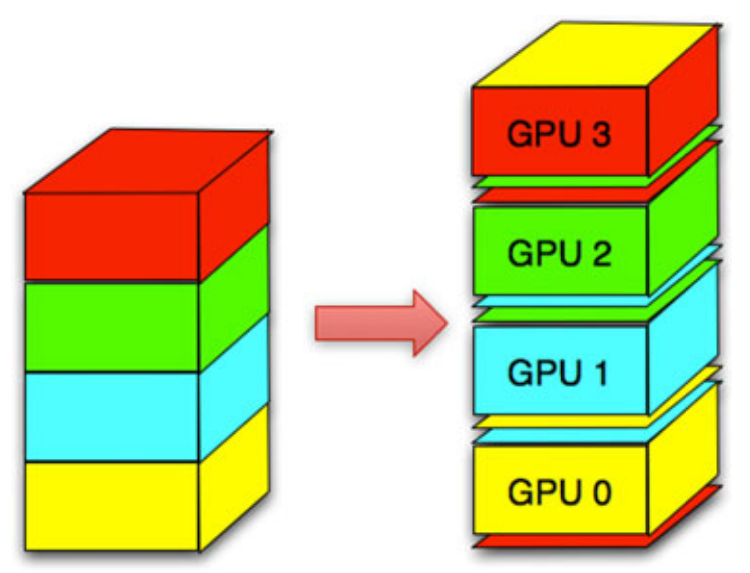
\includegraphics[width=1.0\textwidth]{./images/opencal/multigpu_domain_decomposition.png}
		\caption{Domain decomposition along one axis.}
		\label{fig:multigpu_domain_decomposition}
	\end{center}
\end{figure}

\subsection{Run Configuration}
Each OpenCAL application is attached with a running configuration that is provided by the user or the programmer and describes both which computational resources are going to be used during the execution and how the domain is going to be decomposed.

The running configuration is provided as a file with the following structure:

\begin{mdframed}
\begin{mdframed}[hidealllines=true,backgroundcolor=blue!5]
	\begin{verbatim}
DIM_1 DIM_2 ... DIM_N
NUMBER OF NODES
	\end{verbatim}

\end{mdframed}
\begin{mdframed}[hidealllines=true,backgroundcolor=red!5]
	\begin{verbatim}
IP_NODE_1 NUM_GPU_NODE_1
PLATFORM_NUMBER_1 DEVICE_NUMBER_1 LOAD_1_1
PLATFORM_NUMBER_1 DEVICE_NUMBER_2 LOAD_1_2
	\end{verbatim}
	\begin{center}
	\scalebox{1.2}{$\hdots$}
	\end{center}
	\begin{verbatim}
PLATFORM_NUMBER_1 DEVICE_NUMBER_K1 LOAD_1_K1
PLATFORM_NUMBER_2 DEVICE_NUMBER_1  LOAD_2_1
	\end{verbatim}
	\begin{center}
	\scalebox{1.2}{$\hdots$}
	\end{center}
	\begin{verbatim}
PLATFORM_NUMBER_2 DEVICE_NUMBER_K2 LOAD_2_K2
	\end{verbatim}
	\begin{center}
	\scalebox{1.2}{$\hdots$}
	\end{center}
	\begin{verbatim}
PLATFORM_NUMBER_M1 DEVICE_NUMBER_KM LOAD_M1_KM1
	\end{verbatim}
\end{mdframed}
\begin{mdframed}[hidealllines=true,backgroundcolor=green!5]
	\begin{verbatim}
IP_NODE_2 NUM_GPU_NODE_2
PLATFORM_NUMBER_1 DEVICE_NUMBER_1 LOAD_1_1
PLATFORM_NUMBER_1 DEVICE_NUMBER_2 LOAD_1_2
	\end{verbatim}
	\begin{center}
	\scalebox{1.2}{$\hdots$}
	\end{center}
	\begin{verbatim}
PLATFORM_NUMBER_1 DEVICE_NUMBER_K1 LOAD_1_K1
PLATFORM_NUMBER_2 DEVICE_NUMBER_1 LOAD_2_1
	\end{verbatim}
	\begin{center}
	\scalebox{1.2}{$\hdots$}
	\end{center}
	\begin{verbatim}
PLATFORM_NUMBER_2 DEVICE_NUMBER_K2 LOAD_2_K2
	\end{verbatim}
	\begin{center}
	\scalebox{1.2}{$\hdots$}
	\end{center}
	\begin{verbatim}
PLATFORM_NUMBER_M2 DEVICE_NUMBER_KM LOAD_M2_KM2
	\end{verbatim}
\end{mdframed}
}
\begin{center}
\scalebox{1.5}{$\vdots$}
\end{center}
\begin{mdframed}[hidealllines=true,backgroundcolor=yellow!10]
	\begin{verbatim}
IP_NODE_N NUM_GPU_NODE_N
PLATFORM_NUMBER_1 DEVICE_NUMBER_1 LOAD_1_1
PLATFORM_NUMBER_1 DEVICE_NUMBER_2 LOAD_1_2
...
PLATFORM_NUMBER_1 DEVICE_NUMBER_K1 LOAD_1_K1
PLATFORM_NUMBER_2 DEVICE_NUMBER_1 LOAD_2_1
...
PLATFORM_NUMBER_2 DEVICE_NUMBER_K2 LOAD_2_K2
...
PLATFORM_NUMBER_MN DEVICE_NUMBER_KM LOAD_MN_KM2
	\end{verbatim}
\end{mdframed}
\end{mdframed}
where
\begin{itemize}
	\item The first line describe the size of the domain as a list of sizes for each dimensions.
	\item The second line contains the number of computational nodes. Each node is described and identified by its IP address.
	\item For each node $i$, a line containing its IP address $IP_i$ and the number of devices to be utilized $NUM\_GPU\_NODE_i$.
   \item $NUM\_GPU\_NODE_i$ lines follows, each containing the definition of the devices within node $i$. A device is identified by its \textbf{platform number}, its  \textbf{device number within the platform} and the \textbf{load} parameter which describe the amount of work, assigned to that device.
	 
\end{itemize}


\subsection{Domain Decomposition}
\label{sec:domain_decomposition}
In this preliminary work, the general strategy for dividing work among the available nodes and devices is decomposing the domain along the first dimension listed in the run configuration. The run file has to correctly describe a $1D$ decomposition along the first dimension of the domain. That means that the following has to be always true:
\[
\sum_i^n \sum_p^{m_i} \sum_d^{k_m} LOAD(i,p,k) = DIM\_1
\]
i.e. the sum of the loads has to always match the size of the first dimension of the domain. This ensures that the whole domain is assigned to some device on some node.

The decomposition follows the order in which nodes and devices are listed in the run file. Subsequents portions of not yet decomposed domain are assigned to subsequent (with the respect to the order in which they appear in the file) device. Size of such portion is described by the device load parameter. In order to show how it works consider the following run configuration file:
\begin{mdframed}[hidealllines=true,backgroundcolor=gray!5]
	\begin{verbatim}
16384 16384
2
192.168.1.111 2  
0 0 4096
0 1 4099
192.168.1.222 3
0 0 1200
1 0 3200
1 1 3792
	\end{verbatim}
\end{mdframed}
which defines a $2D$ domain of size $2^{{14}^2} = 2^{28}}$ points.
The domain is scattered along the first dimension, $x$, among 2 nodes and 5 devices, in the following way:
\begin{itemize}
	\item $0 \leq x < 4096 \longmapsto$  device $(0,0)$ running at node $192.168.1.111$.
	\item  $4096 \leq x < 4096+4099$ go to device $(0,1)$ running at node $192.168.1.111$.
	
	\item  $4096+4096\leq x < 1200+4096+4096 \longmapsto$  device $(0,0)$ running at node $192.168.1.222$.
	\item  $1200+4096+4096\leq x < 3200+1200+4096+4096 \longmapsto$  device $(1,0)$ running at node $192.168.1.222$.
	\item  $3200+1200+4096+4096\leq x < 3792+3200+1200+4096+4096 \longmapsto$  device $(1,1)$ running at node $192.168.1.222$.
\end{itemize}



Generally speaking using the decomposition described in section \ref{sec:domain_decomposition} when $N$ devices are involved a GPU $i$ needs to know, for the update of the nodes in its own boundaries, the value of substates belonging to the devices in the boundaries of its neighbors (neighboring device are possibly located in a separate node), so, at each iteration, it must perform all the operations depicted in Figures \ref{fig:communication_scheme} and \ref{fig:multigpu_naive_exchange} (assuming periodic boundary conditions for the sake of simplicity).
\begin{figure}[H]
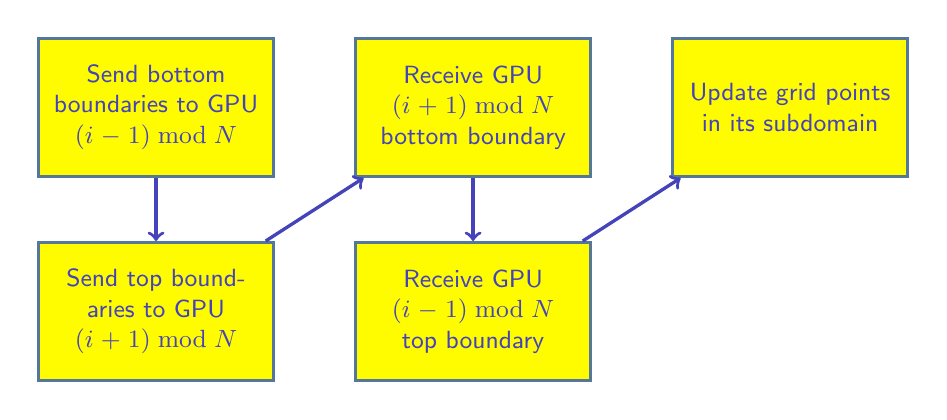
\begin{tikzpicture}
\definecolor{blue1}{HTML}{4443ba}
\definecolor{blue2}{HTML}{55779A}
\definecolor{myyellow}{HTML}{fffc00}
\definecolor{myblue}{HTML}{4443ba}
\matrix [column sep=10mm, row sep=8mm, every node/.style={
	shape=rectangle,
	text width=2.75cm,
	minimum height=1.75cm,
	text centered,
	font=\sffamily\small,
	very thick,
	color=myblue,
	draw=blue2,
	fill=myyellow,
}] {
	\node (a1) {Send bottom boundaries to GPU $(i-1)\bmod N$}; &
	\node (a2) {Receive GPU $(i+1)\bmod N$ bottom boundary}; &
	\node (a3) {Update grid points in its subdomain}; \\
	
	\node (b1) {Send top boundaries to GPU $(i+1)\bmod N$}; &	
	\node (b2) {Receive GPU $(i-1)\bmod N$ top boundary}; &
	\\
};
\begin{scope}[->, very thick, blue1]
\draw (a1) -- (b1);
\draw (b1) -- (a2);
\draw (a2) -- (b2);
\draw (b2) -- (a3);
\end{scope}
\end{tikzpicture}
\label{fig:communication_scheme}
\caption{Communication scheme in a multi-GPU OpenCL application}
\end{figure}

%\begin{enumerate}
%	\item send its bottom boundary to the GPU number $(i-1) \bmod N$
%	\item send its top boundary to the GPU number $(i+1) \bmod N$
%	\item receive $(i+1) \bmod N$ bottom boundary
%	\item receive $(i-1) \bmod N$ top boundary
%	\item update grid points belonging to nodes of its subdomain
%\end{enumerate}

\begin{figure}
	\centering
		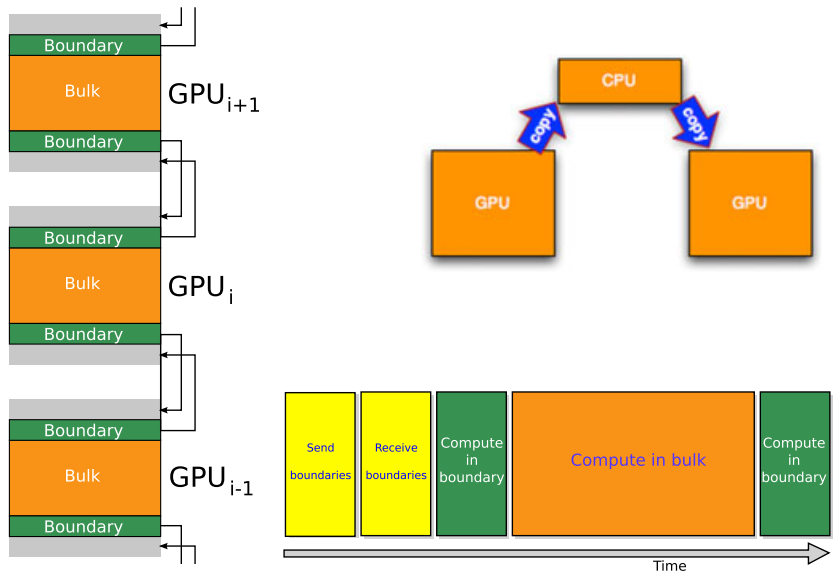
\includegraphics[width=1.0\textwidth]{./images/opencal/multigpu_naive_exchange.png}
		\caption{The adopted Multi-GPU computation scheme.}
		\label{fig:multigpu_naive_exchange}
\end{figure}


Note that this approach always requires CPU intervention as the OpenCL device-device memory transfer feature in the current implementation only works between devices that are within the same OpenCL context. This implies that synchronization is also required during the boundary exchange, as depicted in figure \ref{fig:multigpu_naive_exchange}b.
For a communication step to take place, it is necessary to:
\begin{enumerate}
	\item Pack and upload boundary data to the CPU ( device$\,\mapsto\,$host  memory transfer)
	\item If the two GPUs involved in the communications are controlled by different nodes, an extra communication step over the network is performed between the two nodes. This phase is implemented via MPI \cite{mpiStandard:1994} to ensure and garantee portability and scalability. 
	\item Unpack and upload boundary data to the receipent GPU (host$\,\mapsto\,$device memory transfer).
\end{enumerate}


\section{OpenCAL cluster API}
This section describes the difference between OpenCAL-CL and OpenCAL cluster and discuss the set of the additional API calls that the cluster version exposes.

The Domain Decomposition format described in section \ref{sec:domain_decomposition} is reflected in OpenCAL with the following classes:
\begin{description}
	\item[\texttt{Device}] described by $4$ non-negative integers, two of which identify the device  within the node (using the OpenCL idiom of platform and device numbers) while the rest describe the portion of the subdomain assigned to the specific device.
	\item[\texttt{Node}] containing an IP address, a description of the portion of subdomain assigned to it and finally, a list of \texttt{Device}s installed on the machine that are used for the computation.
	\item [\texttt{Cluster}] containing a list of \texttt{Node}s that are concurrently used to  execute an OpenCAL application.
\end{description}
A \texttt{Cluster} can conveniently constructed from a file using the \texttt{calFromClusterFile} method exposed. It parse, validate and finally return a valid \texttt{Cluster} instance.

\subsection{\texttt{Init} and \texttt{finalize} functors}
The Cluster Abstraction is utilized by the \texttt{MultiNode} class
\lstset{language=[OpenCL]C,frame=tb,
	caption=OpenCAL cluster MultiNode Class Declaration, 
	label=code:multinode, 
	basicstyle=\footnotesize\ttfamily,
	keywordstyle=\color{blue}\ttfamily,
	stringstyle=\color{red}\ttfamily,
	commentstyle=\color{green}\ttfamily,
	backgroundcolor=\color{light-gray}, 
	numbers=left,numbersep=3pt,, 
	\lstset{language=[OpenCL]C,frame=tb,
}
\begin{lstlisting}
template <class Init_Functor,class Finalize_Functor>

class MultiNode{
public:
Cluster c;
Init_Functor *init;
Finalize_Functor *finalize;
...
\end{lstlisting}
which among others fields, contains a \texttt{Cluster} object and two pointers to functors which type is shown in listing \ref{code:init_finalize_signature}.
\lstset{language=[OpenCL]C,frame=tb,
	caption=OpenCAL cluster init and finalize functor signature, 
	label=code:init_finalize_signature, 
	basicstyle=\footnotesize\ttfamily,
	keywordstyle=\color{blue}\ttfamily,
	stringstyle=\color{red}\ttfamily,
	commentstyle=\color{green}\ttfamily,
	backgroundcolor=\color{light-gray}, 
}
\begin{lstlisting}
void finalize(struct CALCLMultiGPU*);
void init(struct CALCLMultiGPU*, const Cluster*);
\end{lstlisting}

\texttt{ init} and \texttt{finalize} if defined, are executed by each MPI process (Node) at the initialization and finalization phases, respectively.
The init functor can be employed to take car of, given the information about the workloads contained into the Cluster object, making sure that each MPI process allocates all of its listed devices with the right resources in order to process the assigned domain.
Devices within a node are managed by a \texttt{CALCLMultiGPU} object,  which  coordinate them and can be created using the \texttt{calclMultiGPUDef2D} API call.
Listing \ref{code:init} shows an example of init function that is part of the Opencal Julia Set generator application shown in section \ref{sec:julia_set} and in listing \ref{code:julia_set}.
\lstset{language=[OpenCL]C,frame=tb,
	caption=OpenCAL cluster finalize example code for the Julia Set generator application. It outputs the node's portion of a substate to a file., 
	label=code:init, 
	basicstyle=\footnotesize\ttfamily,
	keywordstyle=\color{blue}\ttfamily,
	stringstyle=\color{red}\ttfamily,
	commentstyle=\color{green}\ttfamily,
	backgroundcolor=\color{light-gray}, 
	numbers=left,numbersep=3pt,, 
	numberstyle=\tiny
}
\begin{lstlisting}
void init(struct CALCLMultiGPU* multigpu, const Cluster* c){
	//add devices from the cluster configuration
	Node mynode = c->nodes[rank];
	auto devices = mynode.devices;
	struct CALCLDeviceManager* calcl_device_manager = calclCreateManager();
	calclSetNumDevice(multigpu, devices.size());
	for (auto& d : devices) {
		calclAddDevice(multigpu, 
			calclGetDevice(calcl_device_manager, d.num_platform, d.num_device),
			d.workload);
	}
	//create the model	
	struct CALModel2D* host_CA =
	calCADef2D(mynode.workload, mynode.columns, CAL_MOORE_NEIGHBORHOOD_2D, CAL_SPACE_TOROIDAL, CAL_NO_OPT);
	//add the substate
	Q_fractal = calAddSubstate2Di(host_CA);
	//gosh cells radius
	int borderSize = 1;
	calclMultiGPUDef2D(multigpu, host_CA, KERNEL_SRC, KERNEL_INC,
					 borderSize, mynode.devices, c->is_full_exchange());
	calclAddElementaryProcessMultiGPU2D(multigpu, 	KERNEL_LIFE_TRANSITION_FUNCTION);
}
\end{lstlisting}

The finalize functor is executed, if defined, at the end of the computation at the node level. Listing \ref{code:finalize} shows an example in which the \texttt{finalize} is used to save a per node copy of the substate to a file.
\lstset{language=[OpenCL]C,frame=tb,
	caption=OpenCAL cluster init and finalize functor signature, 
	label=code:finalize, 
	basicstyle=\footnotesize\ttfamily,
	keywordstyle=\color{blue}\ttfamily,
	stringstyle=\color{red}\ttfamily,
	commentstyle=\color{green}\ttfamily,
	backgroundcolor=\color{light-gray}, 
	numbers=left,numbersep=3pt,, 
	numberstyle=\tiny\ttfamily\color{gray}
}
\begin{lstlisting}
void finalize(struct CALCLMultiGPU* multigpu){
//for each node, save the substate to a file
std::string fractal_str = "./fractal_portion" + std::to_string(rank)+".txt";
	calSaveSubstate2Di(multigpu->device_models[0]->host_CA, fractal_substate, (char*)fractal_str.c_str());
}
\end{lstlisting}

A MultiNode is used in user code as shown in listing \ref{code:multinode_user_code}
\lstset{language=[OpenCL]C,frame=tb,
	caption=OpenCAL cluster init and finalize functor signature, 
	label=code:init_finalize_signature, 
	basicstyle=\footnotesize\ttfamily,
	keywordstyle=\color{blue}\ttfamily,
	stringstyle=\color{red}\ttfamily,
	commentstyle=\color{green}\ttfamily,
	backgroundcolor=\color{light-gray}, 
}
\begin{lstlisting}
	//Construct a MultiNode object
	MultiNode<decltype(init), decltype(finalize)> mn(cluster, mpi_world_rank, init, finalize);
	//trigger allocation and init execution
	mn.allocateAndInit();
\end{lstlisting}
\section{OpenCAL Cluster High Resolution Julia Set Generation}
\label{sec:opencal_julia}
As a first illustrative example of the usage of OpenCAL cluster this section shows an application which generates high resolution Julia Set images running on an heterogeneous cluster of GPUs.

\subsection{Julia Set}
Julia set fractals are normally generated by initializing a complex number  $z = x + yi$  where  $i2 = -1$  and $x$ and $y$ are image pixel coordinates. Then, $z$ is repeatedly updated using:
\[ 
 z_{n+1} = z_n^2 + c
\]  
where $c$ is a complex constant that gives a specific Julia set (see Figure \ref{julia_set_c}).

\begin{figure}[!htb]
	\minipage{0.32\textwidth}
	\begin{subfigure}{1.0\textwidth}
		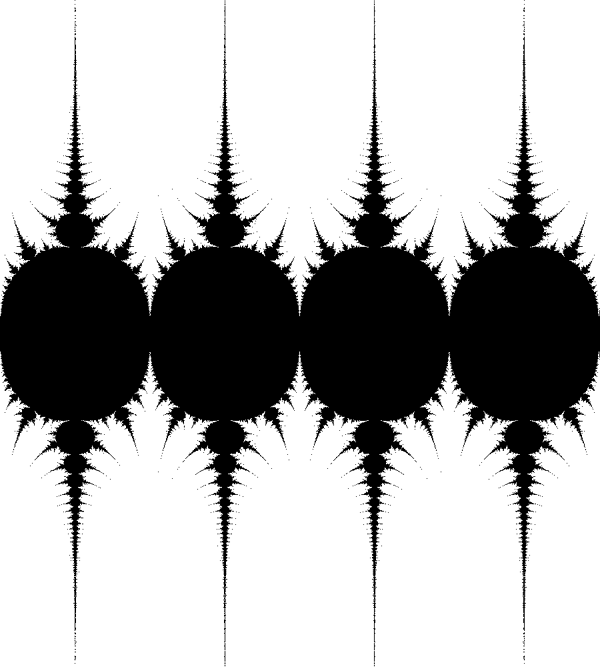
\includegraphics[width=\linewidth]{./images/opencal/julia1.png}
		\label{fig:julia1}
		\caption{$c=1+0i$}
	\end{subfigure}		
	\endminipage\hfill
	\minipage{0.32\textwidth}
	\begin{subfigure}{1.0\textwidth}
		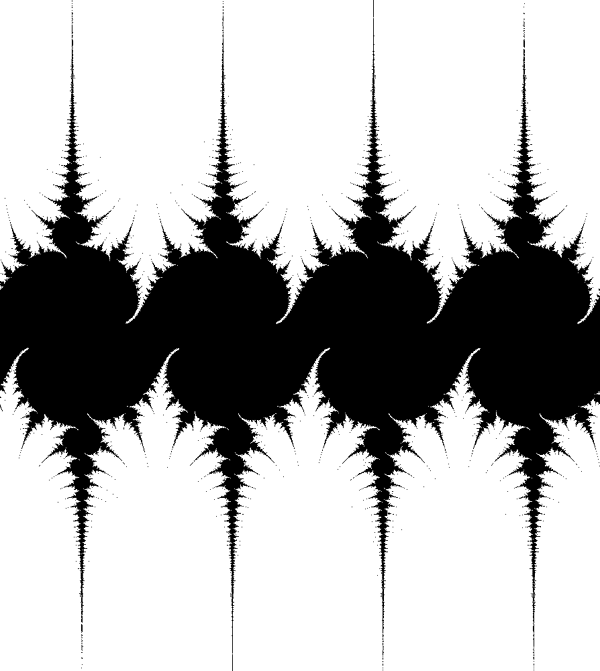
\includegraphics[width=\linewidth]{./images/opencal/julia2.png}
		\label{fig:julia2}
		\caption{$c=1+0.1i$}
	\end{subfigure}
	\endminipage\hfill
	\minipage{0.32\textwidth}%
	\begin{subfigure}{1.0\textwidth}
	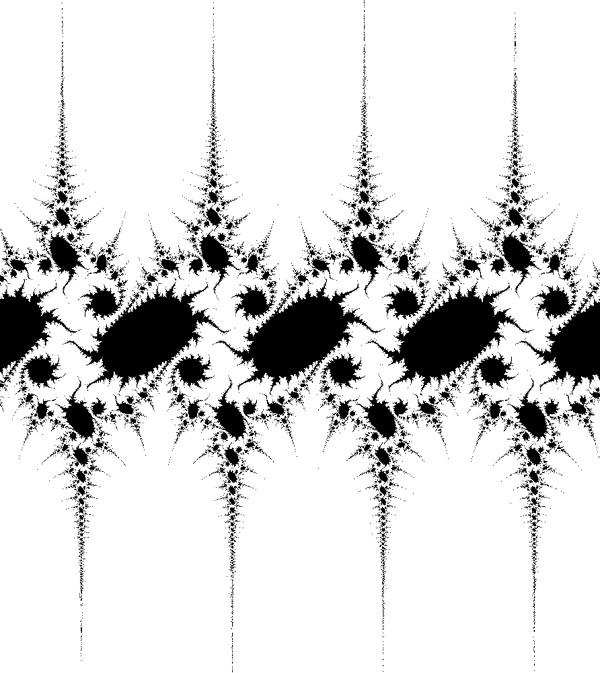
\includegraphics[width=\linewidth]{./images/opencal/julia3.png}
	\label{fig:julia3}
	\caption{$c=1+0.2i$}
\end{subfigure}	
	\endminipage
	\hfill \\ %second row
	\minipage{0.32\textwidth}
		\begin{subfigure}{1.0\textwidth}
		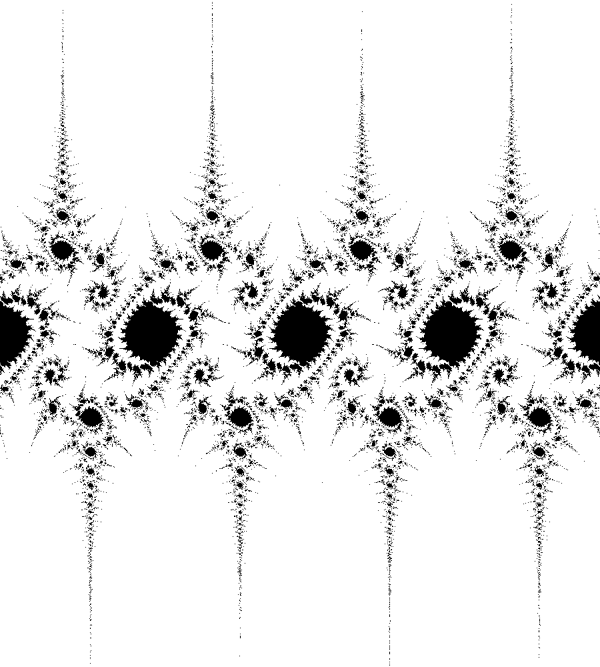
\includegraphics[width=\linewidth]{./images/opencal/julia4.png}
		\label{fig:julia4}
		\caption{$c=1+0.3i$}
	\end{subfigure}
	\endminipage\hfill
	\minipage{0.32\textwidth}
		\begin{subfigure}{1.0\textwidth}
		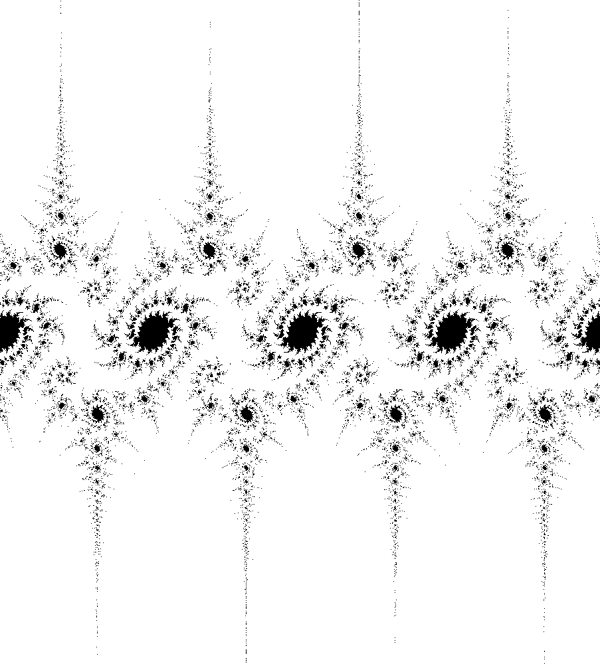
\includegraphics[width=\linewidth]{./images/opencal/julia5.png}
		\label{fig:julia5}
		\caption{$c=1+0.4i$}
	\end{subfigure}
	\endminipage\hfill
	\minipage{0.32\textwidth}%
		\begin{subfigure}{1.0\textwidth}
		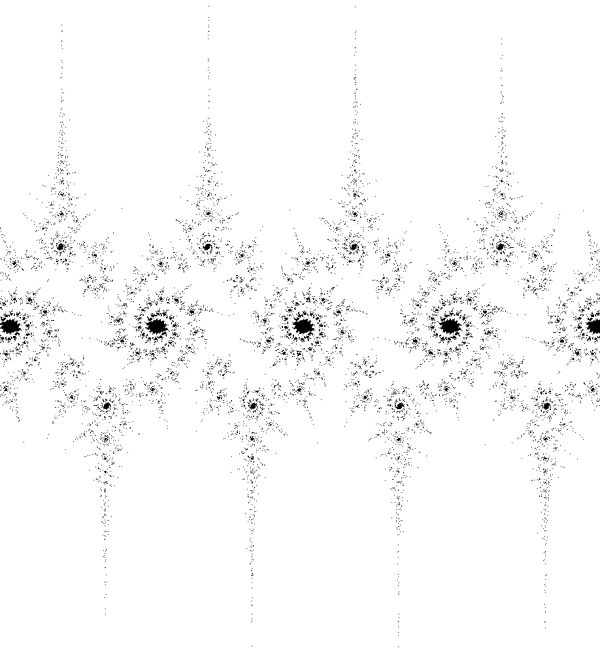
\includegraphics[width=\linewidth]{./images/opencal/julia6.png}
		\label{fig:julia6}
		\caption{$c=1+0.5i$}
	\end{subfigure}
	\endminipage
	\caption{6 Examples of Julia sets obtained variating the constant $c$.}
\end{figure}

In the broader sense the exact for of the iterated function may be almost anything of the form $z_{n+1} = f(z_n)$. Interesting sets arises with non-linear functions. Commonly used ones include the following:
\begin{align*}
z_{n+1} &= c\, sin(z_n) & z_{n+1} &= c \,exp(z_n)\\
z_{n+1} &= i\,c\, cos(z_n) &z_{n+1} &= c\, z_n(1-z_n)
\end{align*}

A point is said to be part of the set if after the repeated iteration does not tent to infinity.
The fractal  is created by first mapping each pixel to a rectangular region of the complex plane. Each pizel represent the initial value of $z_0$. The series is computed for each pixel and if it does not diverge to infinity it is drawn in black, if it doesn't then a color is choosen depending on the number of iteration taken to diverge. This convergence or otherwise isn't always obvious and it may take a large number of iterations to resolve so a decision procedure is required to determine divergence. This typically involves assuming the series tends to infinity as soon as its value exceeds some value, if the series has not diverged after a certain number of terms it is similarly assigned to be part of the set. Both these decisions can be varied to give more precise images but ones that take longer to calculate. 

\subsection{OpenCAL Cluster implementation}
In order to generate the fractal, for each pixel the information regarding how many steps are necessary to diverge is stored in a single integral substate.

As described in section \ref{sec:OpenCAL-CL} every OpenCAL-CL application is divided in a device (kernels) and host side part. 
The iterative process is implemented in listing \ref{code:julia_set} and is run once for each pixel of the final image.
Host side code is shown in listing \ref{code:julia_set_host}. Note that \texttt{init} and \texttt{finalize} functions are omitted since are already shown in listings \ref{code:init} and \ref{code:finalize} at page \pageref{code:init} and \pageref{code:finalize} , respectively.

\lstset{language=[OpenCL]C,frame=tb,
	caption=OpenCAL cluster kernel for the generation of Julia Set., 
	label=code:julia_set_host, 
	basicstyle=\footnotesize\ttfamily,
	keywordstyle=\color{blue}\ttfamily,
	stringstyle=\color{red}\ttfamily,
	commentstyle=\color{green}\ttfamily,
	backgroundcolor=\color{light-gray}, 
	numbers=left,numbersep=3pt,, 
	numberstyle=\tiny\ttfamily\color{gray}
}
\begin{lstlisting}
#define KERNEL_SRC "~/fractal2D/kernel_fractal2D/source/"
#define KERNEL_INC "~/fractal/kernel_fractal2D/include/"
#define KERNEL_LIFE_TRANSITION_FUNCTION "fractal2D_transitionFunction"

struct CALSubstate2Di *Q_fractal; 
int main(int argc, char** argv){
		//create the cluster file from input parameter path
		string clusterfile;
		clusterfile = parseCommandLineArgs(argc, argv);
		Cluster cluster;
		cluster.fromClusterFile(clusterfile);
	    //declare and initialize a multinode object
		MultiNode<decltype(init), decltype(finalize)> mn(cluster, world_rank, init, finalize);
		mn.allocateAndInit();
	    //start crunching numbers
		MPI_Barrier(MPI_COMM_WORLD);
		mn.run(STEPS);
		//a barriere and finalize functor are implicitly called here
	return 0;
}



\end{lstlisting}

\lstset{language=[OpenCL]C,frame=tb,
	caption=OpenCAL cluster kernel for the generation of Julia Set., 
	label=code:julia_set, 
	basicstyle=\footnotesize\ttfamily,
	keywordstyle=\color{blue}\ttfamily,
	stringstyle=\color{red}\ttfamily,
	commentstyle=\color{green}\ttfamily,
	backgroundcolor=\color{light-gray}, 
	numbers=left,numbersep=3pt,, 
	numberstyle=\tiny\ttfamily\color{gray}
}
\begin{lstlisting}
typedef double2  cl_complex;

#define DEVICE_Q_fractal (0)
#define MAXITERATIONS (5000)
#define SIZE (16384)
#define moveX (0)
#define moveY (0)
// Maps and zoom a pixel (x,y) to the complex plane
cl_complex convertToComplex(const int x, const int y, const double zoom,
const int DIMX, const int DIMY) {
	double jx = 1.5 * (x - DIMX / 2.0) / (0.5 * zoom * DIMX) + moveX;
	double jy = (y - DIMY / 2.0) / (0.5 * zoom * DIMY) + moveY;
	return (cl_complex)(jx, jy);
}
cl_complex juliaFunctor(const cl_complex p, cl_complex c) {
	const cl_complex c_ipow =
		cl_complex_multiply(&p, &p); 
	return cl_complex_add(&c_ipow, &c);
}
//Returns the number of iteration taken to diverge to infinity 
int evolveComplexPoint(cl_complex p, cl_complex c) {
	int it = 1;
	while (it <= MAXITERATIONS && cl_complex_modulus(&p) <= 10) {
		p = juliaFunctor(p, c);
		it++;
	}
	return it;
}
__kernel void fractal2D_transitionFunction(__CALCL_MODEL_2D) {
	calclThreadCheck2D();
	int i = calclGlobalRow() + borderSize;
	int j = calclGlobalColumn();
	
	const double zoom = 1.0;
	const cl_complex c;	c.x = -0.391;c.y = -0.587;
	
	int global_i = i - borderSize + offset;
	cl_complex p = convertToComplex(global_i, j, zoom, SIZE, SIZE);
	calclSet2Di(MODEL_2D, DEVICE_Q_fractal, i, j, evolveComplexPoint(p, c));
}
\end{lstlisting}


 \begin{figure}[H]
	\begin{center}
		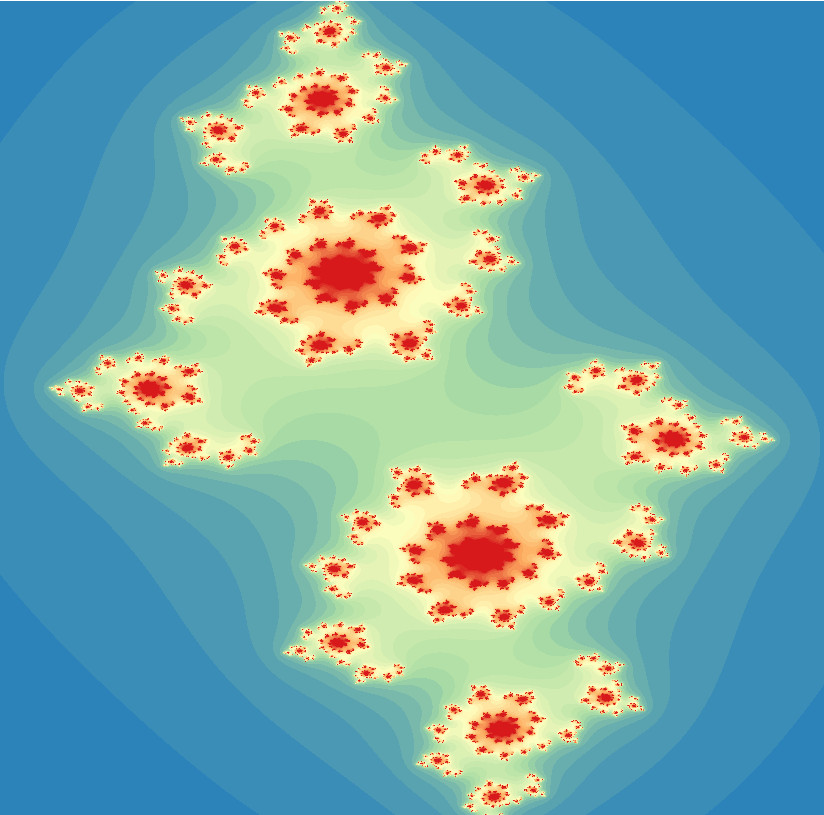
\includegraphics[scale=0.35]{./images/opencal/fractal16k16k}
		\caption{Julia set of size 1.07 GigaPixel, $\approx 3.22 GB$ in the BMP uncompressed format. It is generated using OpenCAL cluster on two \texttt{NVIDIA GTX 980} and rendered on QGIS \cite{QGIS_software} interpreting each point value as color intensity in the spectral color map. Note that the Figure has been subsequently optimized and rescaled for book format.}
		\label{fig:fractal16k16k}
	\end{center}
\end{figure}

\subsection{Convolutional Filters}
The example presented in this section is an application that applies a the sobel convolutional filter on a very large 2D image of size XXX MP. The code presented can be trivially extendend in order to support any kind of convolutional filter on domain of higher dimensions.

 \begin{figure}
	\begin{center}
		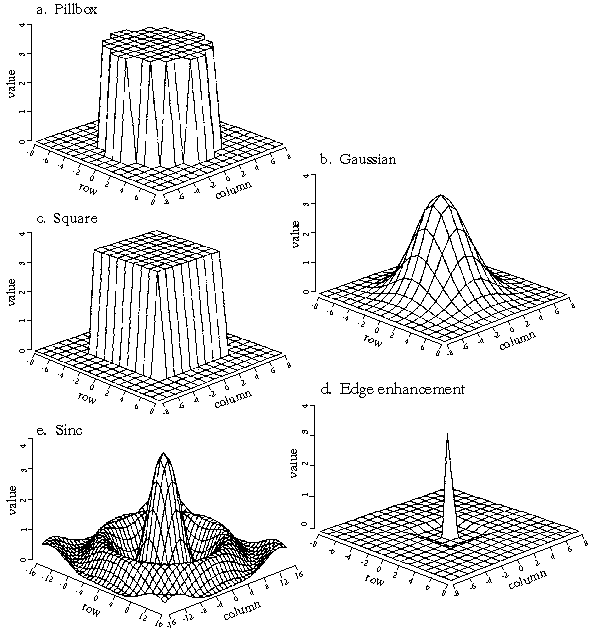
\includegraphics[width=0.72\textwidth]{./images/opencal/kernel_functions}
		\caption{Common point spread functions. The Pillbox (a), Gaussian (b) and Square (c) are common smoothing, low-pass filters. Edge enhancement (d) is an example of high-pass filter. }
		\label{fig:kernel_functions}
	\end{center}
\end{figure}
Convolution filtering is used to modify the spatial frequency
characteristics of an image. Its name derives from the term \textit{convolution} which is a general purpouse filter. It is applied to each  point of the domain and consists of determining the new value of the point  by adding weighted values of all its neighbors together, as shown in Figure \ref{fig:convolution}.
 \begin{figure}
	\begin{center}
		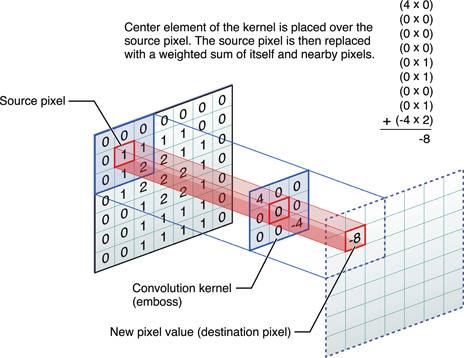
\includegraphics[width=1.0\textwidth]{./images/opencal/kernel_convolution}
		\caption{The process of determining the new value of the central cell by applying a convolution matrix to its neighborhood.}
		\label{fig:convolution}
	\end{center}
\end{figure}
Conovolution is performed multiplying the whole neighborhood of a point by a  matrix, the kernel of the convolution, which usually is a small square matrix of size $r$ (the most common size for kernels is $3\times 3$).
Kernels coefficients correnspond to pointwise values of a arbitrary fixed continuous function, called Point Spread Functions (PFS). Figure \ref{fig:kernel_functions} depicts some of the most common PFS.

Convolution is very often used in image processing. Examples in this field are the Sobel's edge detection filter and the Gaussian Blur filter, that are shown in Figures \ref{fig:sobel} and \ref{fig:gaussian}.

\subsubsection{Edge Handling}
Kernel Convolution requires values from pixels outside the image boundaries. There are a number of ways for handling these corner cases:
\begin{description}
    \item[Wrap] \hfill \\The image is conceptually treated as it was wrapped in a toroidal shape. OpenCAL natively deals with toroidal domain.
    \item[Mirror] \hfill \\
    The image boundaries are mirrored at the edges, maning that if trying to read a pixel 2 units outside the edges, the returned value is the corrensponding pixel 2 unit inside the edge instead.
    \item [Crop]\hfill \\
    	The final image does not contain pixel which would require values from beyond the edges. The output is smaller than the input because edges have been cropped out.
\end{description}

\begin{figure}
	\minipage{0.65\textwidth}
	\begin{subfigure}{1.0\textwidth}
		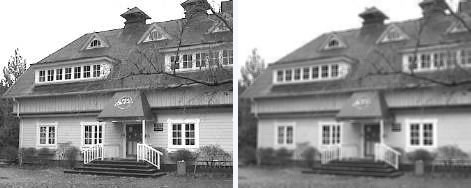
\includegraphics[width=\linewidth]{./images/opencal/gaussian_example}
		
			
	\end{subfigure}
	
	\endminipage\hfill
	\minipage{0.30\textwidth}
	\begin{subfigure}{0.9\textwidth}
		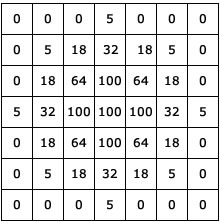
\includegraphics[width=\linewidth]{./images/opencal/conv-gaussian-blur}	
	\end{subfigure}
	\endminipage\hfill
	\caption{Gaussian Convolution filter application. The emnployed Gaussian Kernel has radius $4$.}
	\label{fig:gaussian}
\end{figure}


\begin{figure}[!htb]
	\minipage{0.65\textwidth}
	\begin{subfigure}{1.0\textwidth}
		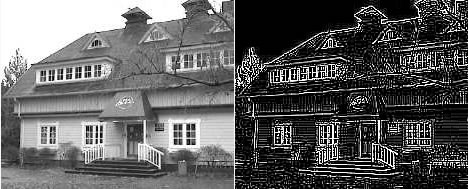
\includegraphics[width=\linewidth]{./images/opencal/sobel_example}
	\end{subfigure}
	
	\endminipage\hfill
	\minipage{0.30\textwidth}
	\begin{subfigure}{1.0\textwidth}
		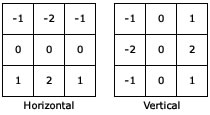
\includegraphics[width=\linewidth]{./images/opencal/conv-sobel}	
	\end{subfigure}
	\endminipage\hfill
	\caption{Sobel edge detection filter. The new pixel value is computed in two subsequent steps, horizontal and vertical, in order the final image to be less affected by noise.}
	\label{fig:sobel}
\end{figure}

Formally convolution can be expressed by the following formula:

\begin{equation*}
   f'_{ij} = \sum_{i'=0}^n (\sum_{j'i'=0}^m f_{(i+i')(j+j')}\times d_{ij})
\end{equation*}
where 
\begin{itemize}
	\item $m,n$ are the  vertical and horizontal size of the kernel,
	\item $f_{ij}$ and $f'_{ij}$ are the old and new value of the cell at coordinate $(i,j)$,
	\item $d_{ij}$ is the value of kernel at location $(i,j)$ 
\end{itemize}


Convolutional filtering is easily implemented in OpenCAL cluster in the following steps and has been applied to the image shown in Figure \ref{fig:sobel_input}:
\begin{enumerate}
    \item Image channels are separately read into OpenCAL \texttt{short} substates (using any image reading third part library, as \texttt{SOIL} \cite{SOIL}, for instance).
    \item A cluster file is defined for the image and shown in listing \ref{code:sobel_cluster_file}. A single node and 3 GPUs were employed in this example. Two \texttt{NVIDIA GTX980} and one \texttt{NVIDIA K40} each with an equal workload.
    \item The kernels depicted in Figure \ref{fig:sobel} are applied to each pixel of the image. OpenCAL kernel code is shown in listing \ref{code:sobel_kernel} 
    \item The resulting image (optimized for book format) is shown in Figure \ref{fig:sobel_result}.
\end{enumerate}

\lstset{language=[OpenCL]C,frame=tb,
	caption=OpenCAL Sobel edge detection filter kernel. For the sake of simplicity, filterting is performed on one color channel only., 
	label=code:sobel_kernel, 
	basicstyle=\footnotesize\ttfamily,
	keywordstyle=\color{blue}\ttfamily,
	stringstyle=\color{red}\ttfamily,
	commentstyle=\color{green}\ttfamily,
	backgroundcolor=\color{light-gray}, 
	numbers=left,numbersep=3pt, 
	numberstyle=\tiny\ttfamily\color{gray}
%	numberstyle=\tiny
}
\begin{lstlisting}
#define DEVICE_Q_red (0)

__kernel void sobel2D_transitionFunction(__CALCL_MODEL_2D) {

calclThreadCheck2D();
int i = calclGlobalRow() + borderSize;
int j = calclGlobalColumn();

CALint sizeOfX_ = calclGetNeighborhoodSize();

int KX[3][3] = {
				{-1, 0, 1},
				{-2, 0, 2},
				{-1, 0, 1}
			   };

int KY[3][3] = {
				{1, 2, 1},
				{0, 0, 0},
				{-1, -2, -1}
			   };

int Gx,Gy,n,k,k1;
Gx = Gy = n = 0;

if (j > 0 && j < calclGetColumns() - 1)
	for (k = -1; k <= 1; k++) {
		for (k1 = -1; k1 <= 1; k1++) {
			Gx += calclGet2Di(MODEL_2D, DEVICE_Q_red, i + k, j + k1) *
													KX[k + 1][k1 + 1];
			Gy += calclGet2Di(MODEL_2D, DEVICE_Q_red, i + k, j + k1) *
													KY[k + 1][k1 + 1];
		}
}

const double R = (Gx * Gx + Gy * Gy);
const int P = sqrt(R);
//set new pixel color for channel red
calclSet2Di(MODEL_2D, DEVICE_Q_red, i, j, P);
return;
}

\end{lstlisting}


\lstset{language=[OpenCL]C,frame=tb,
	caption=Adopted cluster file for the Sobel filtering example. The image is decomposed equally among 3 devices. , 
	basicstyle=\footnotesize\ttfamily,
	label={code:sobel_cluster_file}
}
\begin{lstlisting}[float]
10800 21600
1
192.168.1.111 3
0 0 3600
0 1 3600
0 2 3600
\end{lstlisting}



\begin{figure}
	\minipage{1.0\textwidth}
	\begin{subfigure}{1.0\textwidth}
		\caption{Input Image}
		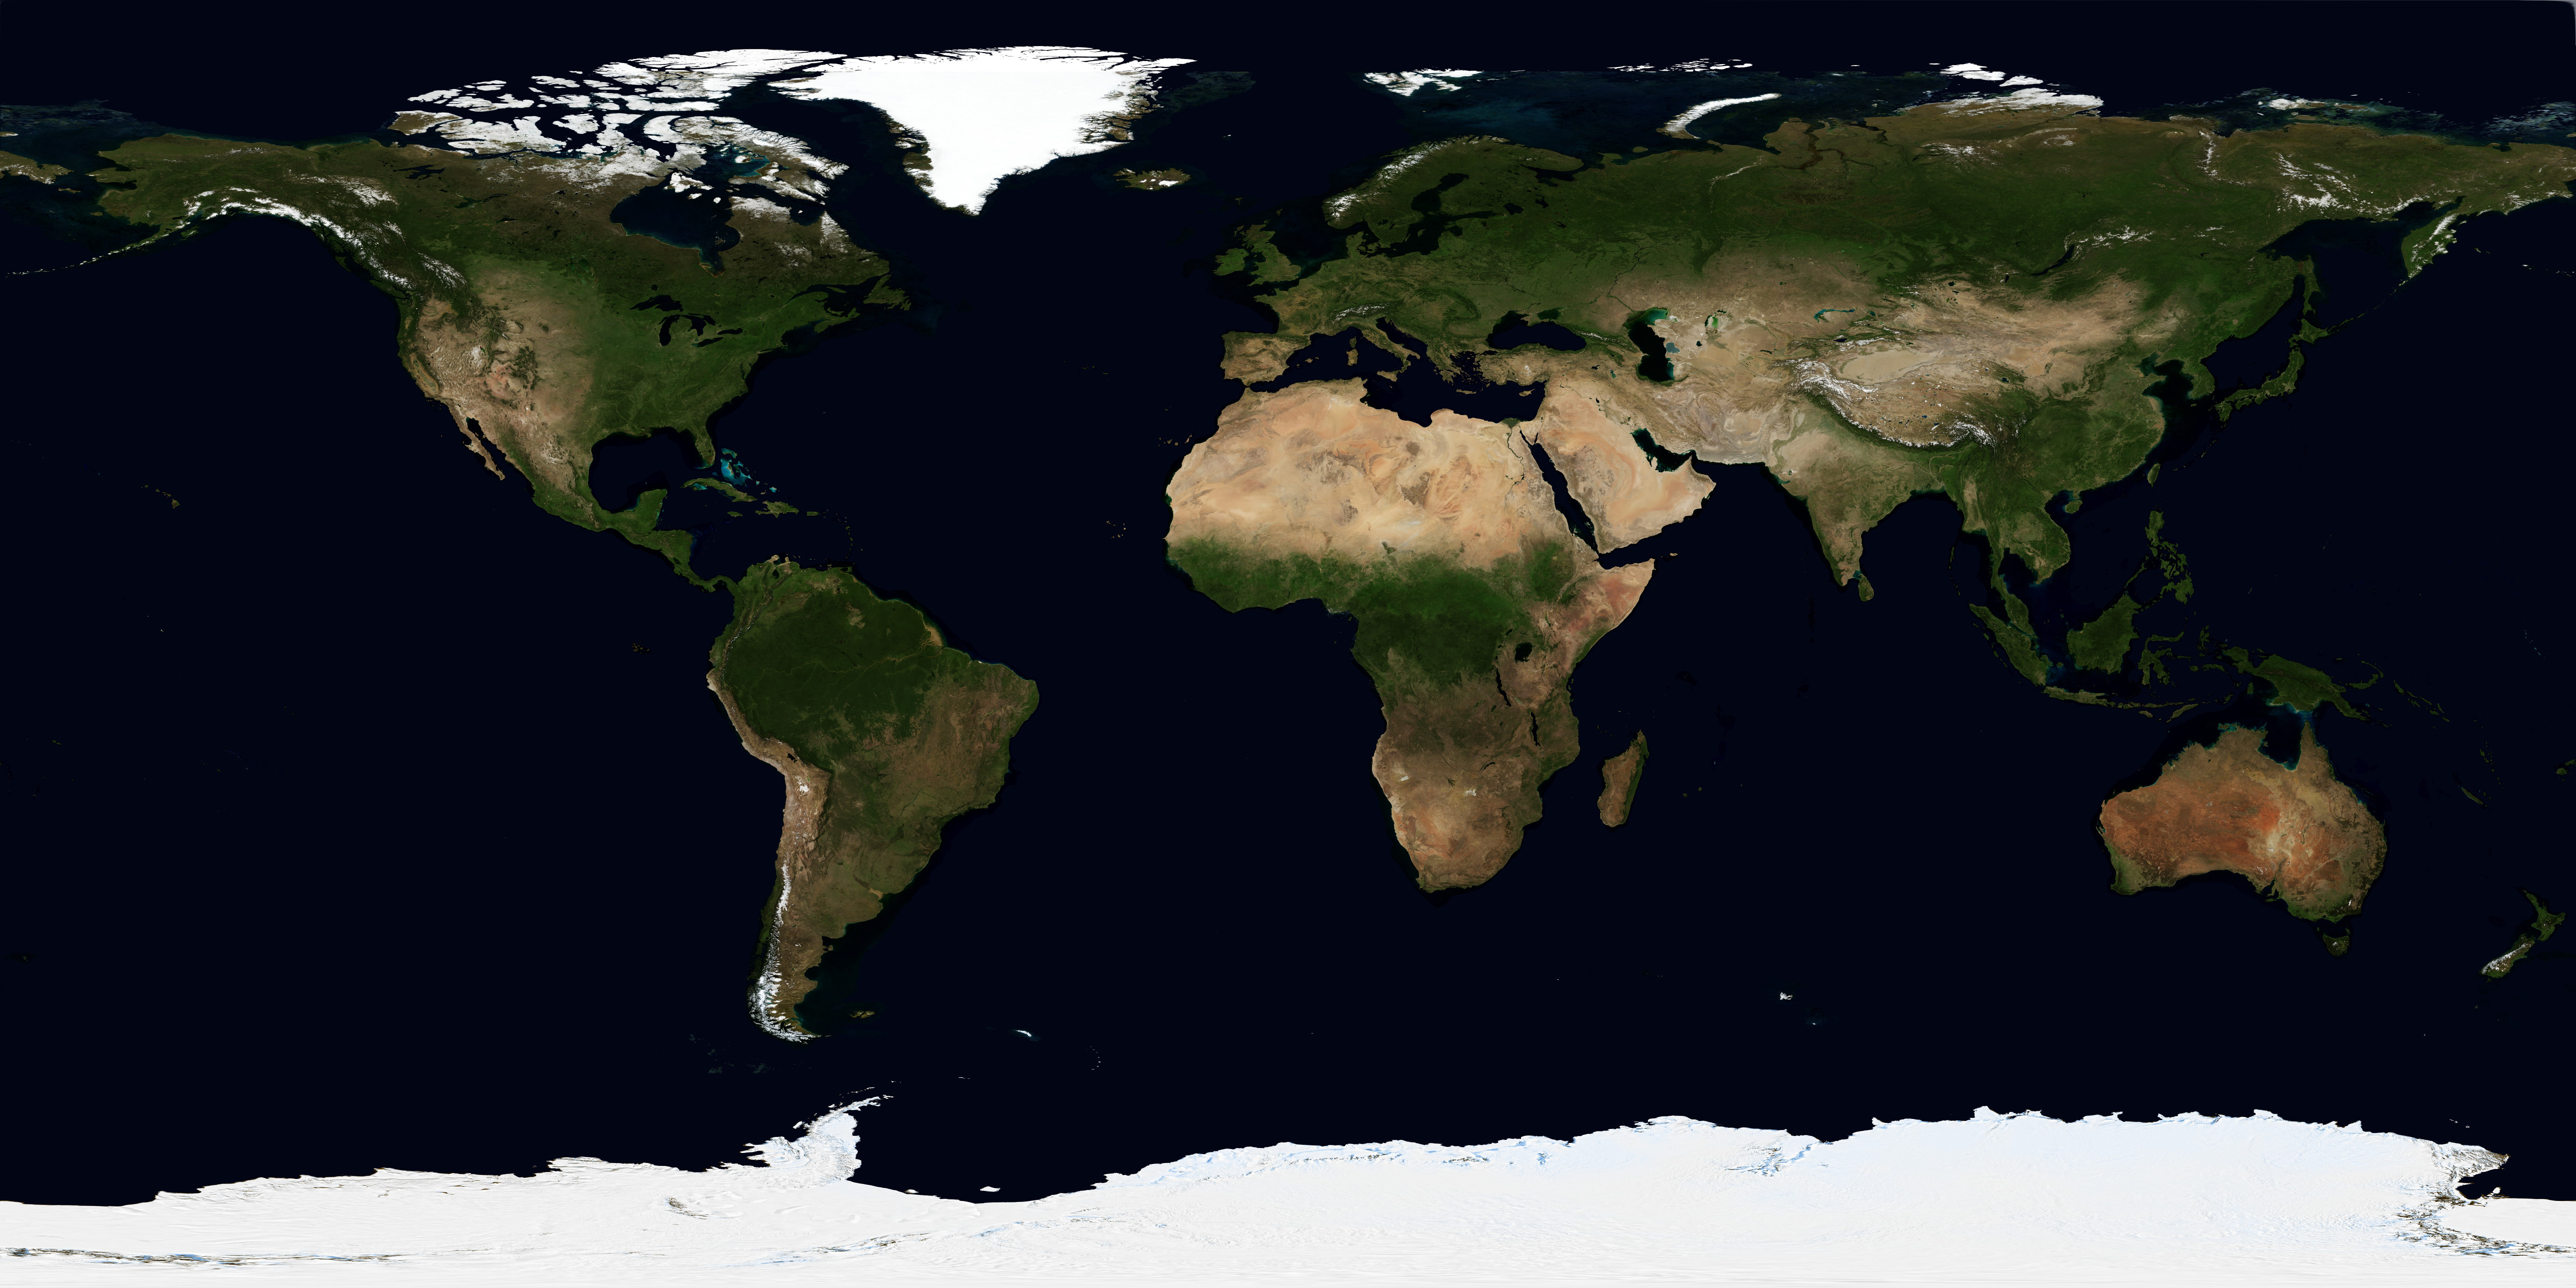
\includegraphics[width=\linewidth]{./images/opencal/sobel_input}
		\label{fig:sobel_input}
		
	\end{subfigure}	
	\endminipage\hfill \\
	\minipage{1.0\textwidth}
		\begin{subfigure}{1.0\textwidth}
		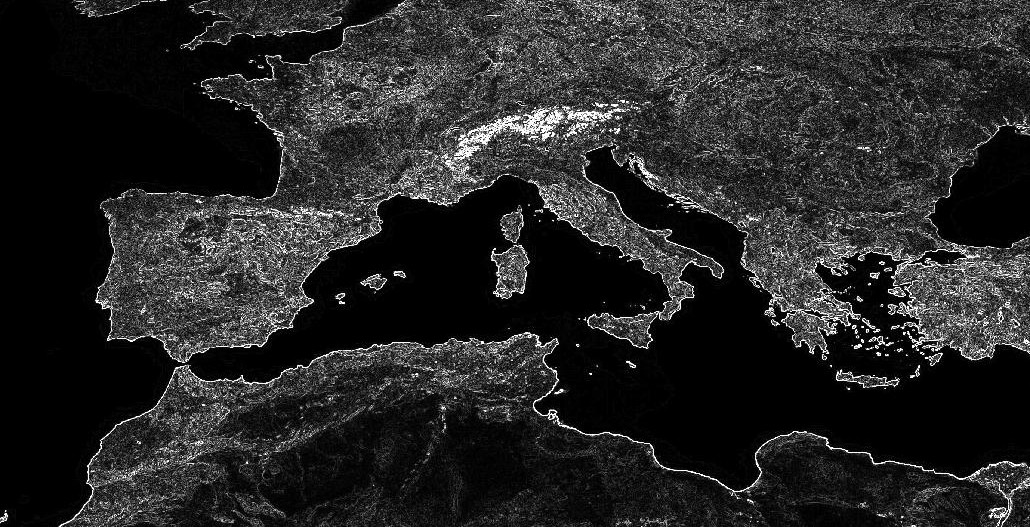
\includegraphics[width=\linewidth]{./images/opencal/sobel_output_detail}
		\label{fig:sobel_output_detail}
		\caption{Zoomed cut on Europe and North Africa of the Output Image.}
	\end{subfigure}
	\endminipage
		\caption{Input Image for the Sobel filter example shown in listing \ref{code:sobel_kernel}. Image size is 233 MegaPixel $\approx 700  \si{MB}$ in \texttt{BMP} uncompressed format.}
		\label{fig:sobel_result}
\end{figure}

commenta tempi di esecuzione e soprattuto che non era possibile arrivato ad un certo punto eseguire nessun filtro perchè la memoria non bastava


\subsection{SciddicaT}




\subsection{Conclusion}
This mechanism is correct and it is the one that is currently implemented in OpenCAL but it is not optimal mainly because of the the serialization of communication and computation and the involvement of the host in each transfer between two GPUs.





\section{blablbl}